\section{Introduction}
\label{sec:ftag-intro}

For the physics program of the ATLAS experiment at the Large Hadron Collider (LHC), the identification of jets initiated by $b$-quarks, or $b$-tagging, is a fundamental tool. 
Ensuring its optimal performance is particularly important for the study of the Higgs boson and the top quark \cite{HIGG-2018-04, HIGG-2018-13}, as well as many exotic extensions of the Standard Model with resonances preferentially decaying to heavy quarks \cite{ATLASdijetres}. 


\begin{figure}[htbp]
  \centering
  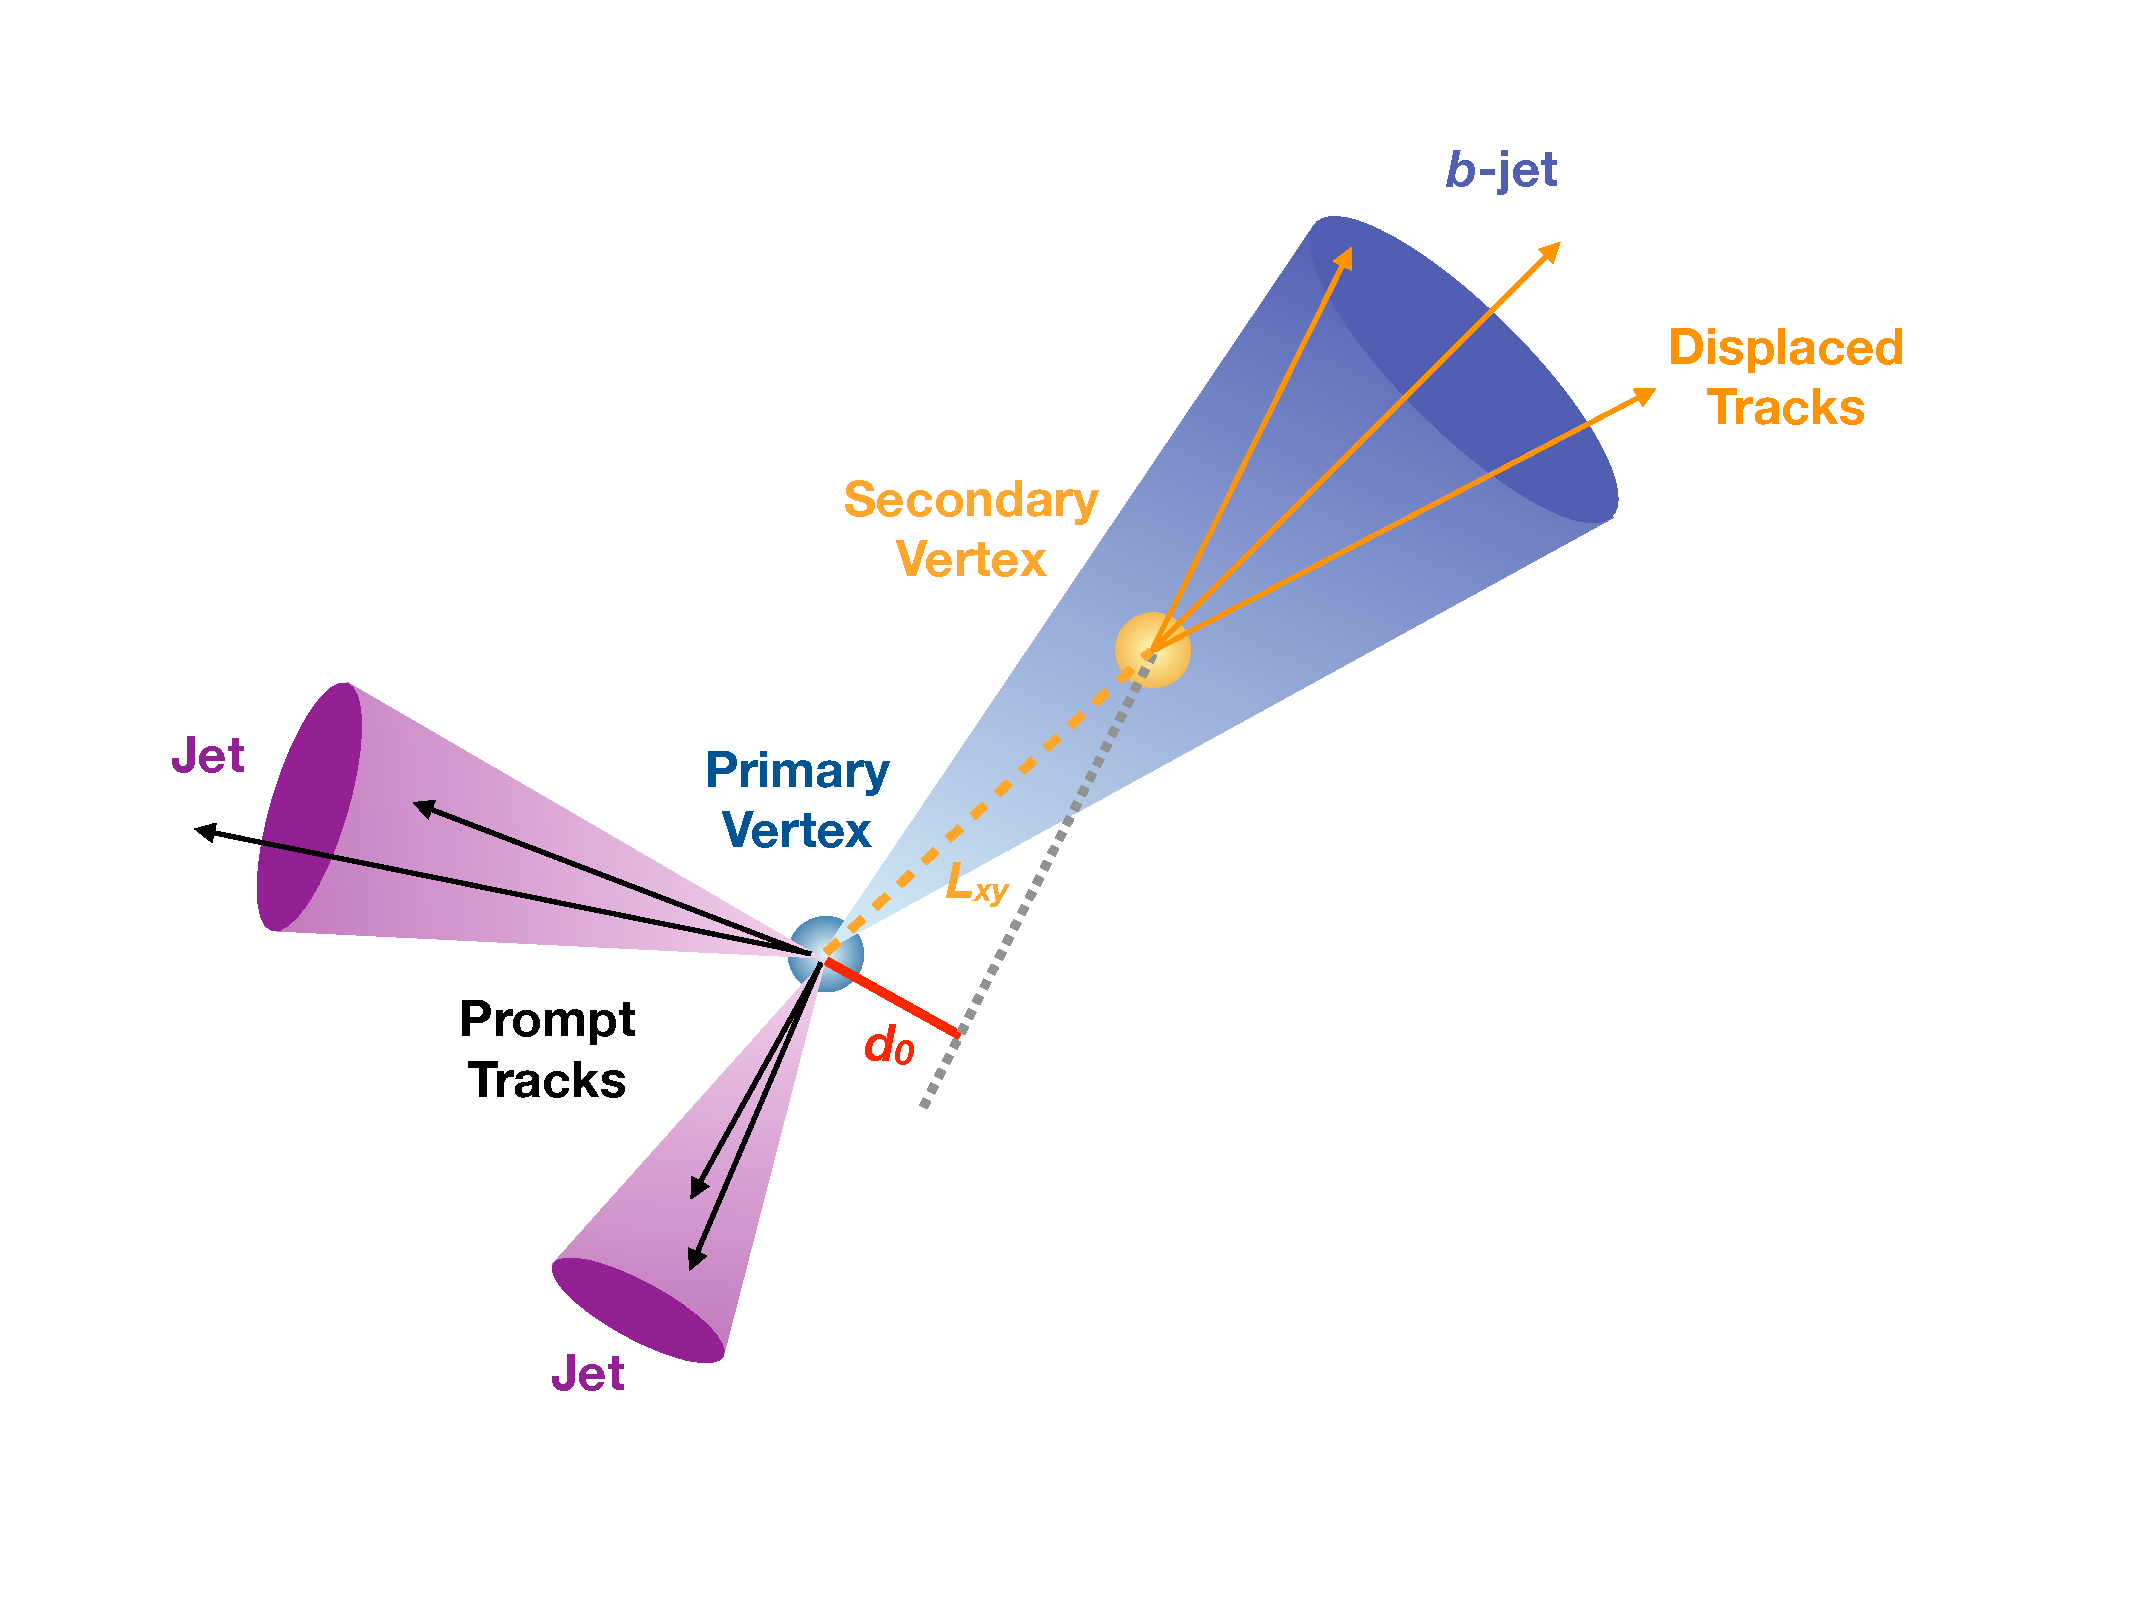
\includegraphics[width=0.7\textwidth]{figures/ftag/b-trig-paper/fig_01}
  \caption{Schematic illustration for the characteristic ``long'' lifetime of a \Pqb-hadron \cite{b-trig-paper}. }
  \label{fig:b-jet-graphic}
\end{figure}

The characteristically long lifetime of hadrons containing $b$-quarks ($b$-hadrons) of the order of 1.5 ps \cite{PDG} leads to two classes of $b$-tagging algorithms: \textit{vertexing} based algorithms which explicitly reconstruct a production point, or vertex, of the $b$-hadron decay displaced from the primary interaction point, and track based algorithms which exploit the displacement of the reconstructed charged particles trajectories (tracks) produced in $b$-hadron decays from the primary interaction point.

%We then use a NN to combine information from these low-level algorithms into a high level tagger and we refer to these collection of algorithm to solve the classification problem of identifying jets containing a $b$-quark as $b$-tagging.

\begin{figure}[htbp]
  \centering
  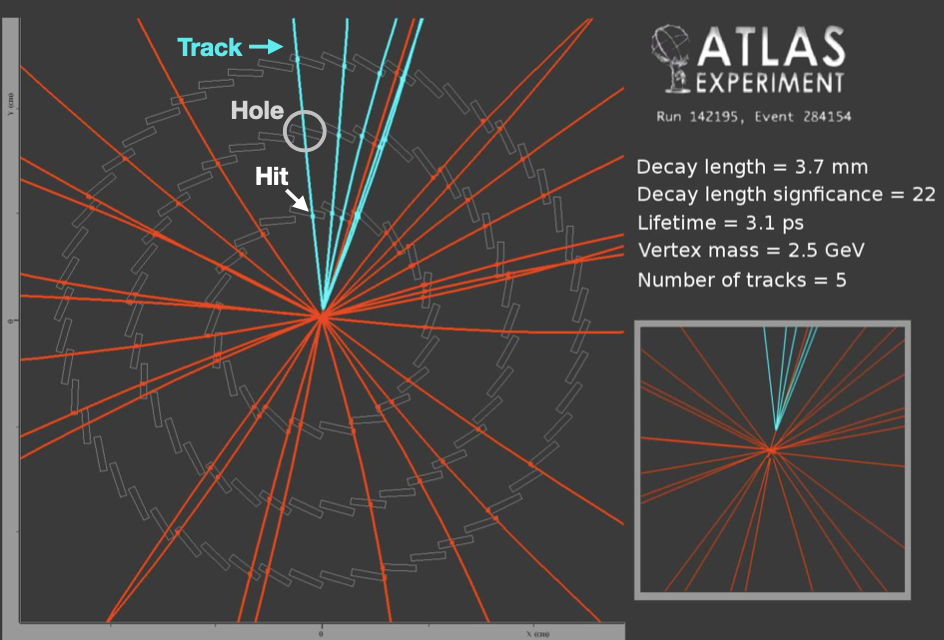
\includegraphics[width=0.9\textwidth]{figures/ftag/b-decay-evt-display-annotated}
  \caption{Illustration of what a b-decay looks like in the ATLAS detector. 
  The cyan colored lines illustrate the tracks from the \Pqb-hadron decay, and in the inset figure you can see the displacement of these tracks from the primary vertex. 
  Only three pixel layers are shown as this is a Run~1 event, and the IBL was not yet installed. \hl{Need to revise older notes to find where this event display came from (or ask Su Dong)}. }
  \label{fig:b-jet-graphic}
\end{figure}

To further set the stage for the problem of interest in this chapter, in \Fig{\ref{fig::jet-displays}} motivates what these weakly decaying hadrons look like in simulation that includes the truth information.
What we have as inputs to flavor tagging are the set of track features in the perigee representation with the IPs defined with respect to the point of closest approach (POCA). \Fig{\ref{fig::jet-displays}} shows these track parameters as we extrapolate out from the PV using the extrapolation equations defined in \Sect{\ref{sec:vertexing}}\footnote{Many thanks to Jonathan Shalomi for the nice track extrapolator code.}.
%The jet displays in \Fig{\ref{fig::jet-displays}} are EMTopo jets passing the standard jet selection cuts, and show all of the reconstructed tracks passing the loosest FTAG preselection. 
These representative images illustrate 
\begin{itemize}
	\item \textbf{\Pqb-jet:} There's a characteristic, tertriary decay of both the B and D hadrons.
	\item \textbf{\Pqc-jet:} There's a weakly decaying D-hadron, but closer to the PV than the weak decays in the \Pqb-jet.
	\item \textbf{light-jet:} Tracks are well collimated with the jet axis and most appear to be originating from the PV, although there are some tracks that that can appear to extrapolate to a point other than the PV.
\end{itemize}

\Tab{\ref{table:decay-length}} shows how often the B and D hadrons decay before the reaching either the first pixel sensor (the IBL) or even the edge of the beam pipe and illustrates that the power of the reconstructing the displaced vertex mostly is coming from the extrapolation.

\begin{table}[h!]
  \centering
    \begin{tabular}{l | l l  } % <-- Alignments: 1st column left, 2nd middle and 3rd right, with vertical lines in between
      {} & \textbf{B-hadron decays before} & \textbf{D-hadron decays before}  \\
      \hline
	Beam pipe &  2.1 \% & 0.3 \% \\
	IBL & 0.94 \% & 0.1 \%
    \end{tabular}
    \caption{Decay length of the weakly decaying hadron for jets in from a semi-leptontic $t\bar{t}$ sample.}
    \label{table:decay-length}
\end{table}

\begin{figure} 
\centering
\vspace{-1cm}
	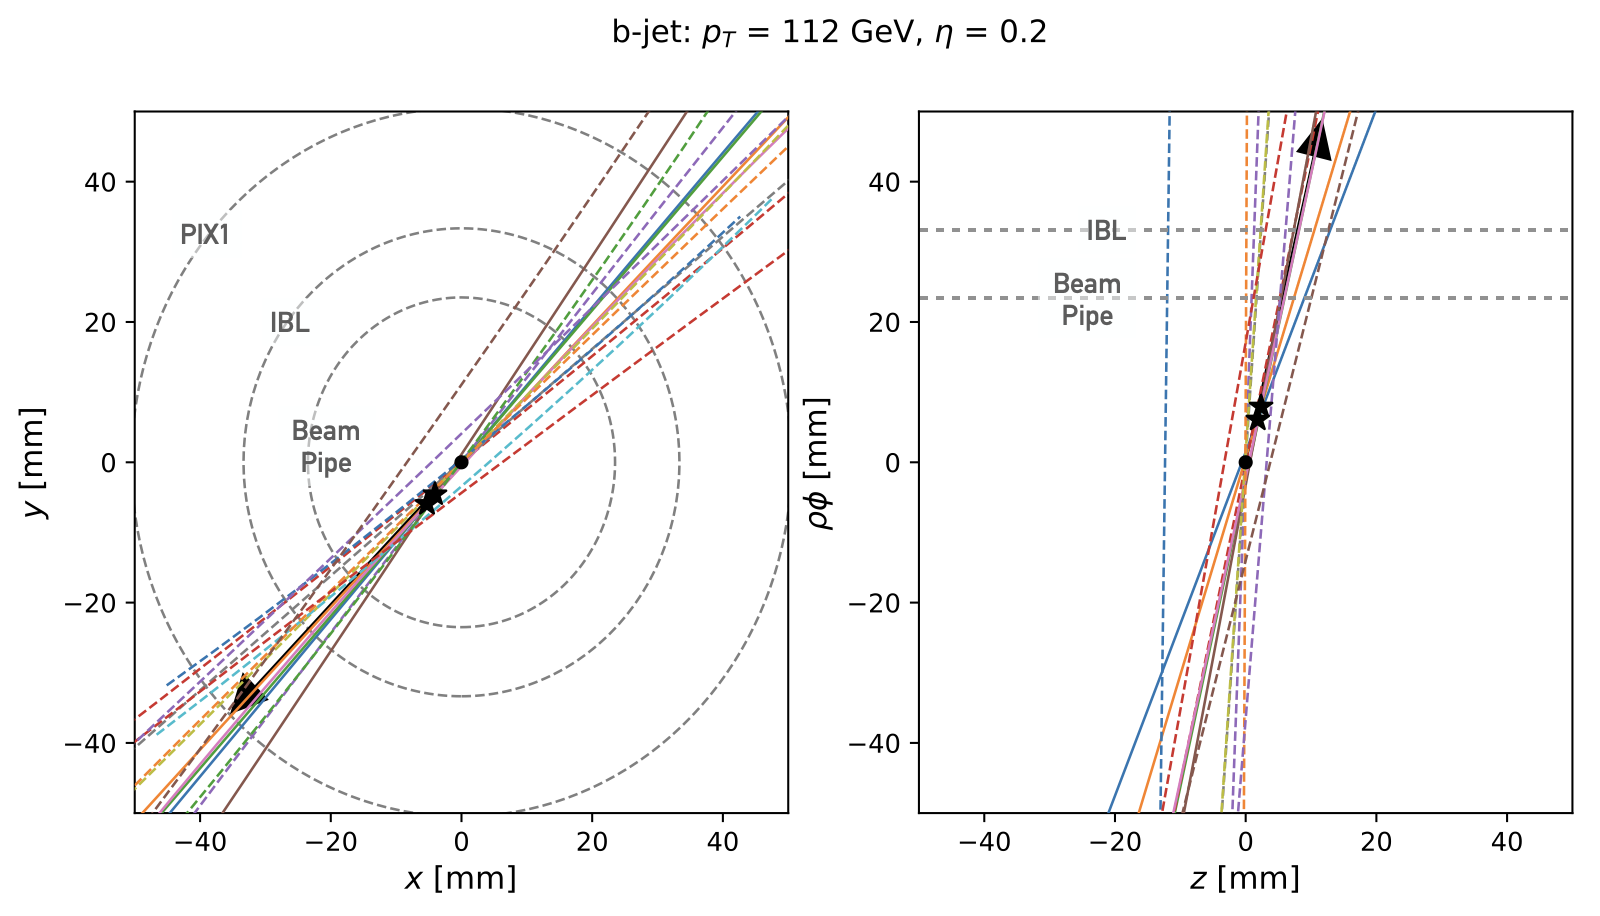
\includegraphics[height=2.75in]{{figures/ftag/jetDisplays/jet5}}
	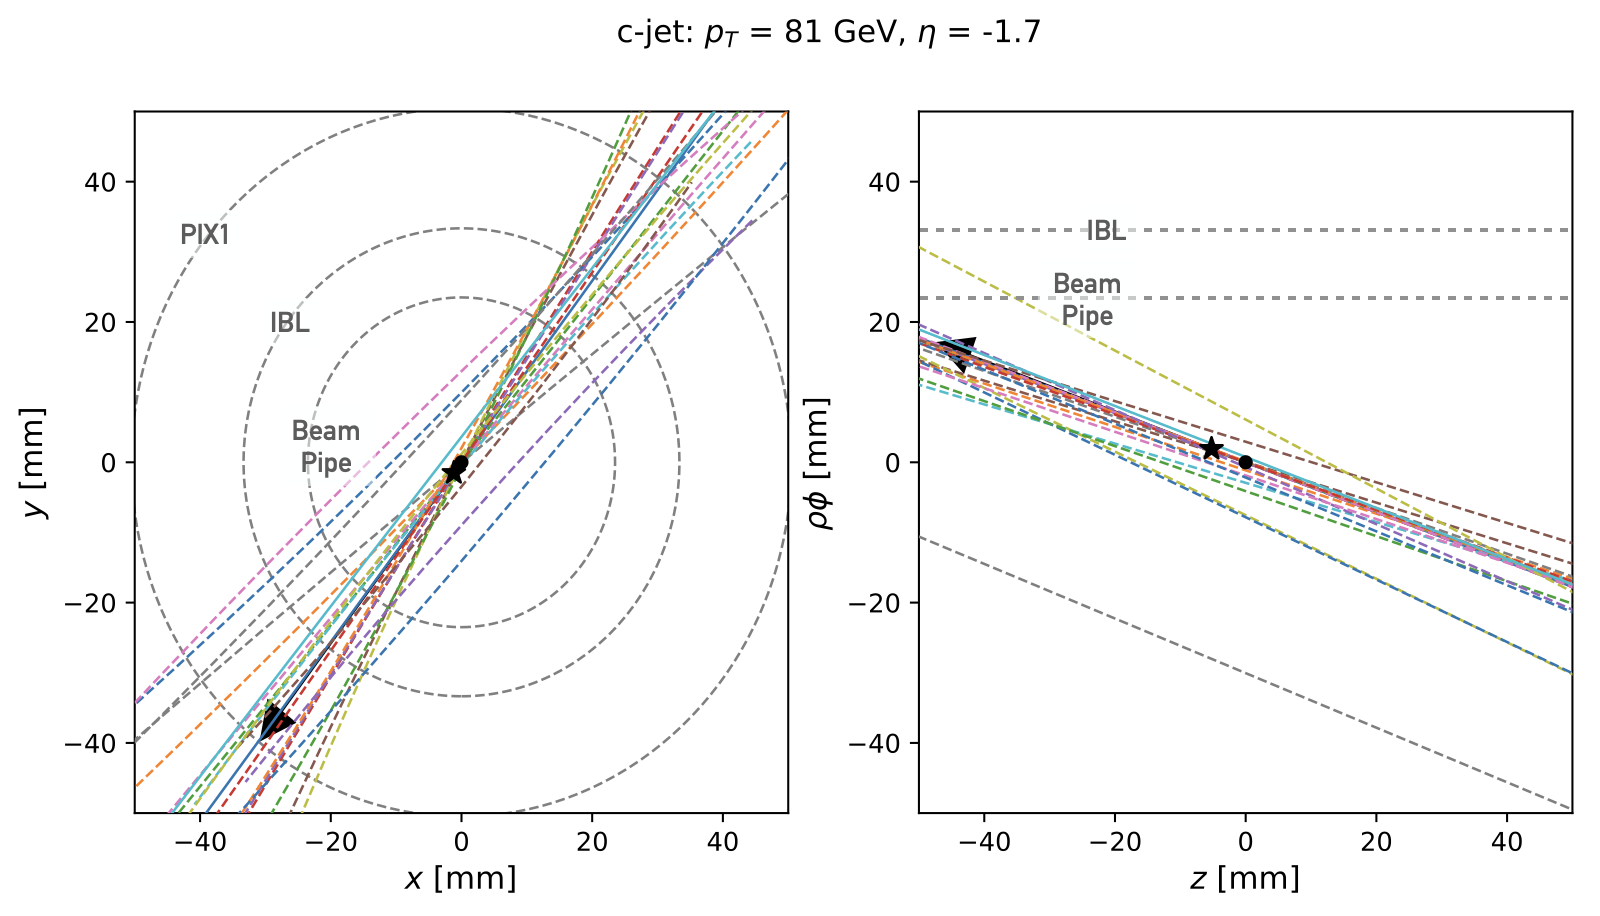
\includegraphics[height=2.75in]{{figures/ftag/jetDisplays/jet32}}
	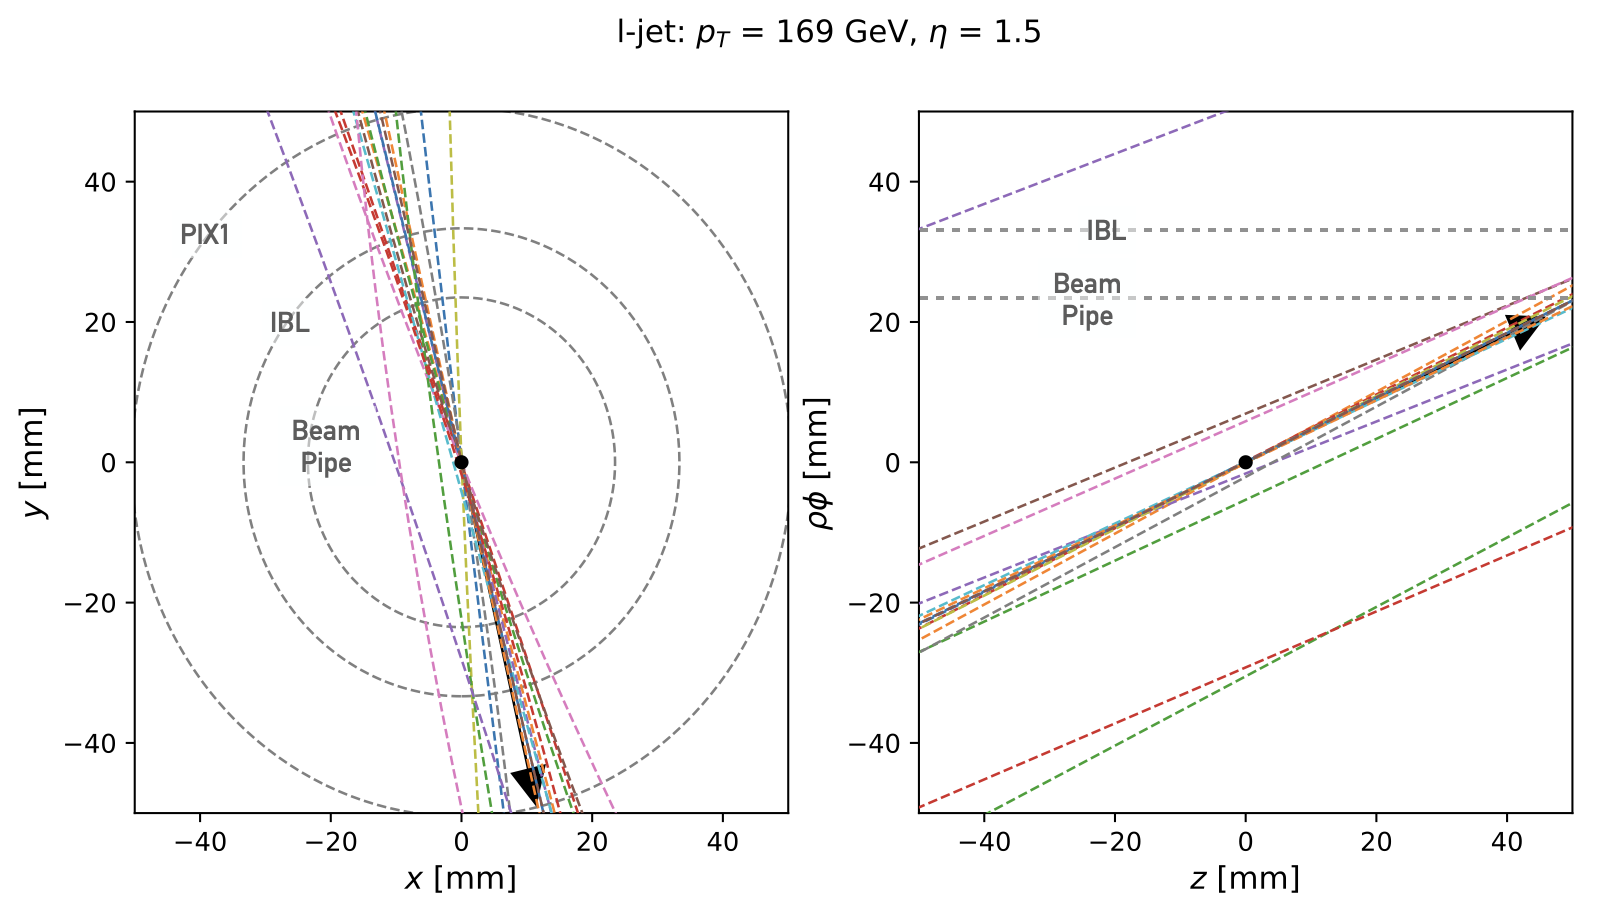
\includegraphics[height=2.75in]{{figures/ftag/jetDisplays/jet3}}
\caption{Visualization of the (x,y) and $(z,\rho\phi)$ 2d views of the tracks for reconstructing the secondary vertex (or vertices). 
The arrow on the figure indicates the jet axis, and a $\star$ shows where the weakly decaying hadron decays.
The solid lines are tracks from the HF decay, while the dashed lines denote the other tracks associated to the jet.}
\label{fig::jet-displays}
\end{figure}

\FloatBarrier
\clearpage

ATLAS employs several IP-based algorithms which are later combined with vertexing algorithms to produce a "high-level" tagger for general use.

\begin{figure}[htbp]
  \centering
  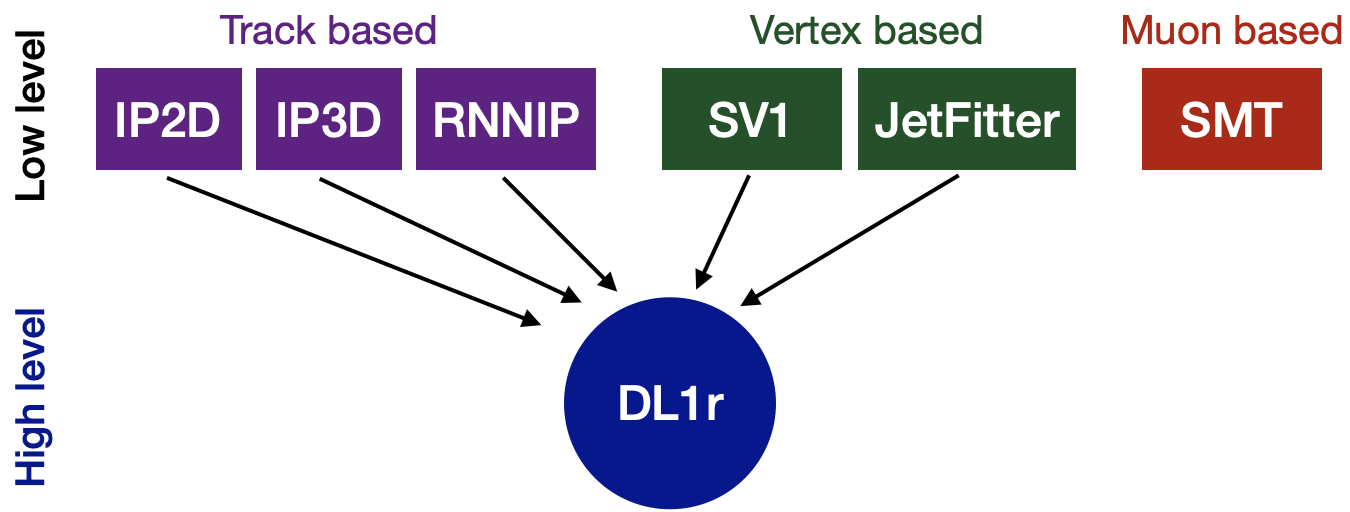
\includegraphics[width=0.9\textwidth]{figures/ftag/ATLAS-taggers}
  \caption{Types of \Pqb-taggers used on ATLAS}
  \label{fig:ATLAS-taggers}
\end{figure}

This chapter is organized as follows: Section \ref{sec:datasets} describes the datasets and selections used to train and evaluate the algorithms, while section \ref{sec:alg} details impact parameter based taggers, the Deep Sets algorithm and our specific implementation. Section \ref{sec:results} shows investigations of what the network has learned, results for the timing metrics, discussion on calibrating the algorithm, and the optimization studies conducted. Finally, section \ref{sec:conclusion} summarizes the conclusions.
